\documentclass{ximera}

%\usepackage{todonotes}

\newcommand{\todo}{}

\usepackage{esint} % for \oiint
\ifxake%%https://math.meta.stackexchange.com/questions/9973/how-do-you-render-a-closed-surface-double-integral
\renewcommand{\oiint}{{\large\bigcirc}\kern-1.56em\iint}
\fi


\graphicspath{
  {./}
  {ximeraTutorial/}
  {basicPhilosophy/}
  {functionsOfSeveralVariables/}
  {normalVectors/}
  {lagrangeMultipliers/}
  {vectorFields/}
  {greensTheorem/}
  {shapeOfThingsToCome/}
  {dotProducts/}
  {partialDerivativesAndTheGradientVector/}
  {../productAndQuotientRules/exercises/}
  {../normalVectors/exercisesParametricPlots/}
  {../continuityOfFunctionsOfSeveralVariables/exercises/}
  {../partialDerivativesAndTheGradientVector/exercises/}
  {../directionalDerivativeAndChainRule/exercises/}
  {../commonCoordinates/exercisesCylindricalCoordinates/}
  {../commonCoordinates/exercisesSphericalCoordinates/}
  {../greensTheorem/exercisesCurlAndLineIntegrals/}
  {../greensTheorem/exercisesDivergenceAndLineIntegrals/}
  {../shapeOfThingsToCome/exercisesDivergenceTheorem/}
  {../greensTheorem/}
  {../shapeOfThingsToCome/}
  {../separableDifferentialEquations/exercises/}
}

\newcommand{\mooculus}{\textsf{\textbf{MOOC}\textnormal{\textsf{ULUS}}}}

\usepackage{tkz-euclide}\usepackage{tikz}
\usepackage{tikz-cd}
\usetikzlibrary{arrows}
\tikzset{>=stealth,commutative diagrams/.cd,
  arrow style=tikz,diagrams={>=stealth}} %% cool arrow head
\tikzset{shorten <>/.style={ shorten >=#1, shorten <=#1 } } %% allows shorter vectors

\usetikzlibrary{backgrounds} %% for boxes around graphs
\usetikzlibrary{shapes,positioning}  %% Clouds and stars
\usetikzlibrary{matrix} %% for matrix
\usepackage{pgfplots}
\usepgfplotslibrary{polar} %% for polar plots
\usepgfplotslibrary{fillbetween} %% to shade area between curves in TikZ
\usetkzobj{all}
\usepackage[makeroom]{cancel} %% for strike outs
%\usepackage{mathtools} %% for pretty underbrace % Breaks Ximera
%\usepackage{multicol}
\usepackage{pgffor} %% required for integral for loops



%% http://tex.stackexchange.com/questions/66490/drawing-a-tikz-arc-specifying-the-center
%% Draws beach ball
\tikzset{pics/carc/.style args={#1:#2:#3}{code={\draw[pic actions] (#1:#3) arc(#1:#2:#3);}}}



\usepackage{array}
\setlength{\extrarowheight}{+.1cm}
\newdimen\digitwidth
\settowidth\digitwidth{9}
\def\divrule#1#2{
\noalign{\moveright#1\digitwidth
\vbox{\hrule width#2\digitwidth}}}





\newcommand{\RR}{\mathbb R}
\newcommand{\R}{\mathbb R}
\newcommand{\N}{\mathbb N}
\newcommand{\Z}{\mathbb Z}

\newcommand{\sagemath}{\textsf{SageMath}}


%\renewcommand{\d}{\,d\!}
\renewcommand{\d}{\mathop{}\!d}
\newcommand{\dd}[2][]{\frac{\d #1}{\d #2}}
\newcommand{\pp}[2][]{\frac{\partial #1}{\partial #2}}
\renewcommand{\l}{\ell}
\newcommand{\ddx}{\frac{d}{\d x}}

\newcommand{\zeroOverZero}{\ensuremath{\boldsymbol{\tfrac{0}{0}}}}
\newcommand{\inftyOverInfty}{\ensuremath{\boldsymbol{\tfrac{\infty}{\infty}}}}
\newcommand{\zeroOverInfty}{\ensuremath{\boldsymbol{\tfrac{0}{\infty}}}}
\newcommand{\zeroTimesInfty}{\ensuremath{\small\boldsymbol{0\cdot \infty}}}
\newcommand{\inftyMinusInfty}{\ensuremath{\small\boldsymbol{\infty - \infty}}}
\newcommand{\oneToInfty}{\ensuremath{\boldsymbol{1^\infty}}}
\newcommand{\zeroToZero}{\ensuremath{\boldsymbol{0^0}}}
\newcommand{\inftyToZero}{\ensuremath{\boldsymbol{\infty^0}}}



\newcommand{\numOverZero}{\ensuremath{\boldsymbol{\tfrac{\#}{0}}}}
\newcommand{\dfn}{\textbf}
%\newcommand{\unit}{\,\mathrm}
\newcommand{\unit}{\mathop{}\!\mathrm}
\newcommand{\eval}[1]{\bigg[ #1 \bigg]}
\newcommand{\seq}[1]{\left( #1 \right)}
\renewcommand{\epsilon}{\varepsilon}
\renewcommand{\phi}{\varphi}


\renewcommand{\iff}{\Leftrightarrow}

\DeclareMathOperator{\arccot}{arccot}
\DeclareMathOperator{\arcsec}{arcsec}
\DeclareMathOperator{\arccsc}{arccsc}
\DeclareMathOperator{\si}{Si}
\DeclareMathOperator{\scal}{scal}
\DeclareMathOperator{\sign}{sign}


%% \newcommand{\tightoverset}[2]{% for arrow vec
%%   \mathop{#2}\limits^{\vbox to -.5ex{\kern-0.75ex\hbox{$#1$}\vss}}}
\newcommand{\arrowvec}[1]{{\overset{\rightharpoonup}{#1}}}
%\renewcommand{\vec}[1]{\arrowvec{\mathbf{#1}}}
\renewcommand{\vec}[1]{{\overset{\boldsymbol{\rightharpoonup}}{\mathbf{#1}}}}
\DeclareMathOperator{\proj}{\mathbf{proj}}
\newcommand{\veci}{{\boldsymbol{\hat{\imath}}}}
\newcommand{\vecj}{{\boldsymbol{\hat{\jmath}}}}
\newcommand{\veck}{{\boldsymbol{\hat{k}}}}
\newcommand{\vecl}{\vec{\boldsymbol{\l}}}
\newcommand{\uvec}[1]{\mathbf{\hat{#1}}}
\newcommand{\utan}{\mathbf{\hat{t}}}
\newcommand{\unormal}{\mathbf{\hat{n}}}
\newcommand{\ubinormal}{\mathbf{\hat{b}}}

\newcommand{\dotp}{\bullet}
\newcommand{\cross}{\boldsymbol\times}
\newcommand{\grad}{\boldsymbol\nabla}
\newcommand{\divergence}{\grad\dotp}
\newcommand{\curl}{\grad\cross}
%\DeclareMathOperator{\divergence}{divergence}
%\DeclareMathOperator{\curl}[1]{\grad\cross #1}
\newcommand{\lto}{\mathop{\longrightarrow\,}\limits}

\renewcommand{\bar}{\overline}

\colorlet{textColor}{black}
\colorlet{background}{white}
\colorlet{penColor}{blue!50!black} % Color of a curve in a plot
\colorlet{penColor2}{red!50!black}% Color of a curve in a plot
\colorlet{penColor3}{red!50!blue} % Color of a curve in a plot
\colorlet{penColor4}{green!50!black} % Color of a curve in a plot
\colorlet{penColor5}{orange!80!black} % Color of a curve in a plot
\colorlet{penColor6}{yellow!70!black} % Color of a curve in a plot
\colorlet{fill1}{penColor!20} % Color of fill in a plot
\colorlet{fill2}{penColor2!20} % Color of fill in a plot
\colorlet{fillp}{fill1} % Color of positive area
\colorlet{filln}{penColor2!20} % Color of negative area
\colorlet{fill3}{penColor3!20} % Fill
\colorlet{fill4}{penColor4!20} % Fill
\colorlet{fill5}{penColor5!20} % Fill
\colorlet{gridColor}{gray!50} % Color of grid in a plot

\newcommand{\surfaceColor}{violet}
\newcommand{\surfaceColorTwo}{redyellow}
\newcommand{\sliceColor}{greenyellow}




\pgfmathdeclarefunction{gauss}{2}{% gives gaussian
  \pgfmathparse{1/(#2*sqrt(2*pi))*exp(-((x-#1)^2)/(2*#2^2))}%
}


%%%%%%%%%%%%%
%% Vectors
%%%%%%%%%%%%%

%% Simple horiz vectors
\renewcommand{\vector}[1]{\left\langle #1\right\rangle}


%% %% Complex Horiz Vectors with angle brackets
%% \makeatletter
%% \renewcommand{\vector}[2][ , ]{\left\langle%
%%   \def\nextitem{\def\nextitem{#1}}%
%%   \@for \el:=#2\do{\nextitem\el}\right\rangle%
%% }
%% \makeatother

%% %% Vertical Vectors
%% \def\vector#1{\begin{bmatrix}\vecListA#1,,\end{bmatrix}}
%% \def\vecListA#1,{\if,#1,\else #1\cr \expandafter \vecListA \fi}

%%%%%%%%%%%%%
%% End of vectors
%%%%%%%%%%%%%

%\newcommand{\fullwidth}{}
%\newcommand{\normalwidth}{}



%% makes a snazzy t-chart for evaluating functions
%\newenvironment{tchart}{\rowcolors{2}{}{background!90!textColor}\array}{\endarray}

%%This is to help with formatting on future title pages.
\newenvironment{sectionOutcomes}{}{}



%% Flowchart stuff
%\tikzstyle{startstop} = [rectangle, rounded corners, minimum width=3cm, minimum height=1cm,text centered, draw=black]
%\tikzstyle{question} = [rectangle, minimum width=3cm, minimum height=1cm, text centered, draw=black]
%\tikzstyle{decision} = [trapezium, trapezium left angle=70, trapezium right angle=110, minimum width=3cm, minimum height=1cm, text centered, draw=black]
%\tikzstyle{question} = [rectangle, rounded corners, minimum width=3cm, minimum height=1cm,text centered, draw=black]
%\tikzstyle{process} = [rectangle, minimum width=3cm, minimum height=1cm, text centered, draw=black]
%\tikzstyle{decision} = [trapezium, trapezium left angle=70, trapezium right angle=110, minimum width=3cm, minimum height=1cm, text centered, draw=black]


\outcome{Use ``shortcut'' rules to find and use derivatives.}
\outcome{Use the definition of the derivative to develop a shortcut
  rule to find the derivative of the sine function.}

\title[Dig-In:]{The derivative of sine}

\begin{document}
\begin{abstract}
  We derive the derivative of sine.
\end{abstract}
\maketitle

It is now time to visit our two friends who concern themselves
periodically with triangles and circles. In particular, we want to show that
\[
\dd{\theta}\sin(\theta)=\cos(\theta).
\]
Before we tackle this monster, let's remember a fact, and derive a new
fact. You may initially be uncomfortable because you can't quite see why we need
these results, but this style of exposition is a fact of technical writing; it
is best to get used to it.

First, recall the fact that
\[
\lim_{\theta\to 0} \frac{\sin(\theta)}{\theta} = 1. %% BADBAD I'd like to link this
\]
Next, we will use this fact to derive our new fact:
\begin{example}
  \[
\lim_{\theta\to 0}\frac{\cos(\theta)-1}{\theta} = 0.
  \]
  \begin{explanation}
    Write with me:
\begin{align*}
\lim_{\theta\to 0}\frac{\cos(\theta)-1}{\theta} &= \lim_{\theta\to 0}\left(\frac{\cos(\theta)-1}{\theta}\cdot\frac{\cos(\theta)+1}{\cos(\theta)+1}\right)\\
&=\lim_{\theta\to 0}\frac{\cos^2(\theta)-1}{\theta(\cos(\theta)+1)}\\
&=\lim_{\theta\to 0}\frac{-\sin^2(\theta)}{\theta(\cos(\theta)+1)}\\
&=-\lim_{\theta\to 0}\left(\frac{\sin(\theta)}{\theta}\cdot\frac{\sin(\theta)}{\cos(\theta)+1}\right)\\
&=-\lim_{\theta\to 0}\answer[given]{\frac{\sin(\theta)}{\theta}} \cdot \lim_{\theta\to 0}\frac{\sin(\theta)}{\cos(\theta)+1}\\
&= -1 \cdot \answer[given]{\frac{0}{2}} = 0.
\end{align*}
  \end{explanation}
\end{example}

After these delicious appetizers, we are now ready for the main course.

\begin{theorem}[The derivative of sine]\index{derivative!of sine}\label{theorem:deriv sin}
For any angle $\theta$ measured in radians, the derivative of $\sin(\theta)$ with respect to $\theta$ is $\cos(\theta)$.  In other words, 
\[
\dd{\theta} \sin(\theta) = \cos(\theta).
\]
\begin{explanation}
Using the definition of the derivative, write with me
\[
\dd{\theta} \sin(\theta) = \lim_{h\to0} \frac{\sin(\theta+h)-\sin(\theta)}{h}
\]
Now we get sneaky and apply the trigonometric addition formula for sine, that says $\sin(\alpha+\beta) = \sin(\alpha)\cos(\beta)+\sin(\beta)\cos(\alpha)$, to write
\begin{align*}
  &= \lim_{h\to0} \frac{\sin(\theta)\cos(h)+\sin(h)\cos(\theta)-\sin(\theta)}{h}  \\
  &= \lim_{h\to0} \left(\frac{\sin(\theta)\cos(h)-\sin(\theta)}{h} + \frac{\sin(h)\cos{\theta}}{h} \right)\\
  &=\lim_{h\to0} \left(\sin (\theta)\frac{\cos(h) - 1}{h}+\cos(\theta)\frac{\sin(h)}{h}\right) \\
   &=\lim_{h\to0} \sin (\theta)\frac{\cos(h) - 1}{h}+\lim_{h\to0}\cos(\theta)\frac{\sin(h)}{h} \\
     &= \sin (\theta)\lim_{h\to0}\frac{\cos(h) - 1}{h}+\cos(\theta)\lim_{h\to0}\frac{\sin(h)}{h} \\
  &=\sin(\theta) \cdot \answer[given]{0} + \cos(\theta) \cdot \answer[given]{1}\\
  &= \cos(\theta). 
\end{align*}
\end{explanation}
\end{theorem}

\begin{question}
  What is the slope of the line tangent to the graph of $\sin(\theta)$ at $\theta =
  \pi/4$?
  \begin{prompt}
    \[
    \answer{\sqrt{2}/2}
    \]
  \end{prompt}
  \begin{explanation}
  The slope of the line tangent to the graph of $\sin(\theta)$ at $\theta =
  \pi/4$ is given by 
  \[
 \eval{\ddx\sin(\theta)}_{\theta= \pi/4}=\cos(\pi/4)=\sqrt{2}/2. 
  \]

    \end{explanation}
\end{question}

For your intellectual stimulation, consider the following geometric
interpretation of the derivative of $\sin(\theta)$.
%\begin{figure}

\begin{image}
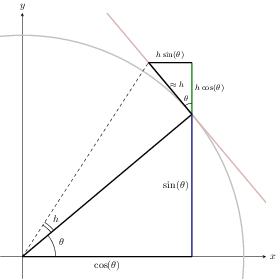
\includegraphics{0.png}
\iffalse
\begin{tikzpicture}
	\begin{axis}[
            xmin=-.1,xmax=1.1,ymin=-.1,ymax=1.1,
            axis lines=center,
            ticks=none,
            width=5in,
            unit vector ratio*=1 1 1,
            xlabel=$x$, ylabel=$y$,
            every axis y label/.style={at=(current axis.above origin),anchor=south},
            every axis x label/.style={at=(current axis.right of origin),anchor=west},
          ]        
          \addplot [very thick, textColor!30!background, smooth, domain=(-.2:.2+pi/2)] ({cos(deg(x))},{sin(deg(x))});
          \addplot [textColor,very thick] plot coordinates {(0,0) (.766,.643)}; %% 40 degrees
          \addplot [textColor,very thick] plot coordinates {(0,0) (.766,0)}; %% bottom
          \addplot [very thick, penColor2!30!background] {(x-.766)*(-.766/.643)+.643};
          \addplot [textColor,dashed] plot coordinates {(0,0) (.766-.196,.643+1-.766)}; %% 40+16.98 degrees          

          %% \addplot [textColor!20!background] plot coordinates {(.766,.643) (1,.839)}; %% hyp
          %% \addplot [textColor!20!background] plot coordinates {(1,.643) (1,.839)}; %% side
          %% \addplot [textColor!20!background] plot coordinates {(.766,.643) (1,.643)}; %% bottom
          %% \addplot [textColor!20!background,smooth, domain=(0:40)] ({.05*cos(x)+.766},{.05*sin(x)+.643}); %% angle
          %% \node at (axis cs:.84,.670) [textColor!20!background] {\footnotesize$\theta$};
          
          %% \addplot [textColor!20!background] plot coordinates {(.766,.643) (.766,.839)}; %% side
          %% \addplot [textColor!20!background] plot coordinates {(.766,.839) (1,.839)}; %% bottom
          %% \addplot [textColor!20!background,smooth, domain=(180:220)] ({.05*cos(x)+1},{.05*sin(x)+.839}); %% angle
          %% \node at (axis cs:.926,.812) [textColor!20!background] {\footnotesize$\theta$};
          
          \draw[rotate around={30:(.5,.5)}] (.7,.7) rectangle (.25,.25);

          %\draw[textColor, rotate around={45:(.5,.5)}] (.5,.5) rectangle (.2,.2);

          \addplot [penColor4,very thick] plot coordinates {(.766,.643) (.766,.643+1-.766)}; %% side
          \addplot [textColor,very thick] plot coordinates {(.766,.643+1-.766) (.766-.196,.643+1-.766)}; %% top
          \addplot [textColor,smooth, domain=(90:130)] ({.05*cos(x)+.766},{.05*sin(x)+.643}); %% angle
          \addplot [very thick, textColor] plot coordinates {(.766-.196,.643+1-.766) (.766,.643)}; %% hyp
          \node at (axis cs:.739,.717) [textColor] {\footnotesize$\theta$};
          
          \node at (axis cs:.668,.877) [anchor=south] {\footnotesize$h\sin(\theta)$};
          \node at (axis cs:.766,.76) [anchor=west] {\footnotesize$h\cos(\theta)$};
          \node at (axis cs:.65,.78) [anchor=west] {\footnotesize$\approx h$};

          \addplot [very thick, penColor] plot coordinates {(.766,0) (.766,.643)}; %% sin theta          
          
          \addplot [textColor, smooth, domain=(0:40)] ({.15*cos(x)},{.15*sin(x)});
          \addplot [textColor, smooth, domain=(40:56.90)] ({.17*cos(x)},{.17*sin(x)});
          \addplot [textColor, smooth, domain=(40:56.90)] ({.185*cos(x)},{.185*sin(x)});
          \node at (axis cs:.15,.07) [anchor=west] {$\theta$};
          \node at (axis cs:.15,.17) {$h$};
          \node at (axis cs:.766,.322) [anchor=east] {$\sin(\theta)$};
          \node at (axis cs:.383,0) [anchor=north] {$\cos(\theta)$};
        \end{axis}
\end{tikzpicture}
\fi
\end{image}
%\label{figure:geo-interp sinx/x}
%\end{figure}

From this diagram, we see that increasing $\theta$ by a small
amount $h$ increases $\sin(\theta)$ by approximately
$h\cos(\theta)$. Hence,
\[
\frac{\Delta y}{\Delta \theta}\approx \frac{h\cos(\theta)}{h} =
\cos(\theta).
\]

With all of this said, the derivative of a function measures the slope
of the plot of a function.  If we examine the graphs of the sine and
cosine side by side, it should be clear that the latter appears to
accurately describe the slope of the former, and indeed this is true.
\begin{image}
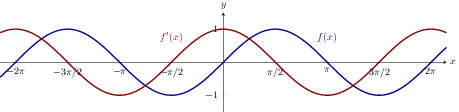
\includegraphics{1.png}
\iffalse
\begin{tikzpicture}
	\begin{axis}[
            xmin=-6.75,xmax=6.75,ymin=-1.5,ymax=1.5,
            axis lines=center,
            xtick={-6.28, -4.71, -3.14, -1.57, 0, 1.57, 3.142, 4.71, 6.28},
            xticklabels={$-2\pi$,$-3\pi/2$,$-\pi$, $-\pi/2$, $0$, $\pi/2$, $\pi$, $3\pi/2$, $2\pi$},
            ytick={-1,1},
            %ticks=none,
            width=9in,
            height=2in,
            unit vector ratio*=1 1 1,
            xlabel=$x$, ylabel=$y$,
            every axis y label/.style={at=(current axis.above origin),anchor=south},
            every axis x label/.style={at=(current axis.right of origin),anchor=west},
          ]        
          \addplot [very thick, penColor, samples=100,smooth, domain=(-6.75:6.75)] {sin(deg(x))};
          \addplot [very thick, penColor2, samples=100,smooth, domain=(-6.75:6.75)] {cos(deg(x))};
          \node at (axis cs:3.14,.75) [penColor] {$f(x)$};
          \node at (axis cs:-1.57,.75) [penColor2] {$f'(x)$};
        \end{axis}
\end{tikzpicture}
%% \caption{Here we see a plot of $f(x)=\sin(x)$ and its derivative
%%   $f'(x)=\cos(x)$. One can readily see that $\cos(x)$ is positive when
%%   $\sin(x)$ is increasing, and that $\cos(x)$ is negative when
%%   $\sin(x)$ is decreasing.}
%% \label{figure:sin/co
%%  s}
\fi
\end{image}

\begin{question}
 Using the graph above, what is the value of $x$ in the interval $[0, 2\pi]$ where the tangent to the graph of $f(x) = \sin(x)$ has slope $-1$?
 \begin{prompt}
   The tangent line to the graph of the function $\sin(x)$ has slope $-1$ at $x = \answer{\pi}$.
 \end{prompt}
\end{question}

Pro-tip: When working with trigonometric functions, you should always
keep their graphical representations in mind.

\end{document}
